% This is samplepaper.tex, a sample chapter demonstrating the
% LLNCS macro package for Springer Computer Science proceedings;
% Version 2.20 of 2017/10/04
%
\documentclass[runningheads]{llncs}
%
\usepackage{graphicx}
\usepackage{amsmath}
\usepackage{amssymb}
\usepackage{bm}
\usepackage{amsfonts}
\usepackage{subfig}
\usepackage{cleveref}
\graphicspath{{./imgs/}}

\begin{document}
%
\title{Normalizing Flows}
%
%\titlerunning{Abbreviated paper title}
% If the paper title is too long for the running head, you can set
% an abbreviated paper title here
%
\author{Abdul Fatir Ansari \and
Devamanyu Hazarika\and
Remmy A. M. Zen}
%
\authorrunning{CS6202 Project Report - Normalizing Flows}
% First names are abbreviated in the running head.
% If there are more than two authors, 'et al.' is used.
%
\institute{National University of Singapore \\
\email{\{abdulfatir,devamanyu,remmy\}@u.nus.edu}}
%
\maketitle              % typeset the header of the contribution
%
\begin{abstract}


\keywords{Normalizing flows \and .}
\end{abstract}
%
%
%
\section{Introduction}
\section{Background}
\subsection{Autoencoder}
\subsection{Variational Autoencoder}


\section{Normalizing Flows}

Before defining normalizing flows, let's consider a univariate distribution with density function $p(x)$. Define a continuous, differentiable, and increasing function $f$. Define $y = f(x)$ where $x \sim p(x)$. The density function of the random variable $Y$ can then be derived analytically using the Cumulative Distribution Function (CDF) as follows.

\begin{align}
F_{Y}(y) &= P(Y \leq y)\\
&= P(f(X) \leq y)\\
&= P(X \leq f^{-1}(y)) = F_{X}( f^{-1}(y))
\end{align}

We end up with the CDF of the random variable $X$ at the point $f^{-1}(y)$. Now, $p(y) = F_{Y}'(y)$ by definition, where

\begin{align}
F_{Y}(y) = F_{X}( f^{-1}(y)) = \int_{-\infty}^{ f^{-1}(y)}p(x) dx
\label{eq:cdfy}
\end{align}

Differentiating Eq. (\ref{eq:cdfy}) with respect to $y$ (using the Fundamental Theorem of Calculus and the chain rule) we get

\begin{align}
p(y) = p(f^{-1}(y))\cdot \frac{df^{-1}}{dy}
\label{eq:incfn}
\end{align}

When $f$ is a decreasing function, we get $p(y) = p(f^{-1}(y))\cdot \frac{df^{-1}}{dy}$.  For an invertible function in general, Eq. (\ref{eq:incfn}) can be written as 

\begin{align}
p(y) = p(f^{-1}(y))\cdot \left|\frac{df^{-1}}{dy}\right|
\label{eq:covuv}
\end{align}

Eq. (\ref{eq:covuv}) can be extended to the multivariate case where the derivative is replaced by the determinant of the Jacobian matrix $J$

\begin{align}
p(\mathbf{y}) = p(f^{-1}(\mathbf{y}))\cdot \left|\det\frac{\partial f^{-1}}{\partial\mathbf{y}}\right| = p(f^{-1}(\mathbf{y}))\cdot \left|\det\frac{\partial f}{\partial f^{-1}(\mathbf{y})}\right|^{-1}
\label{eq:covmv}
\end{align}

In the above equation, the second equality comes from the inverse function theorem. Successive applications of such smooth, invertible transformation on a random variable with known density is called a \textit{normalizing flow}.

 Computation of the probability density of the transformed random variable requires the computation of the determinant of the Jacobian matrix which is computationally expensive as it scales with $O(d^3)$ where $d$ is the dimensionality of the random variable. Developing transformations with cheap determinant computation has been the primary focus of many recent works.
\section{Applications}
Literature on normalizing flows can be broadly classified into two parts: ones using normalizing flows for improved variational inference and ones using normalizing flows for density estimation.
\subsection{Variational Inference}
Variational methods perform inference by approximating the true posterior $p(z|x)$ using a simpler variational family $q_{\phi}(z|x)$. Recent works have focused on improving the variational posterior used in the VAE which is generally set to a multivariate normal distribution with diagonal covariance matrix $\mathcal{N}(\bm{\mu}, \sigma^2\mathbf{I})$. It is clear that such a simplistic, unimodal choice for the posterior can be arbitrarily far away from the true posterior which can be a complex multi-modal distribution. 

Recent works seek to convert samples from a simple variational posterior (such as the multivariate normal distribution) into a richer distribution by applying a series of smooth, invertible transformations or a flow. Let $\mathbf{z}_0$ be a sample from a simple distribution $q_0(\mathbf{z}_0)$ and $\mathbf{z}_K$ be a sample obtained by applying a flow of length $K$ on $\mathbf{z}_0$, i.e., $\mathbf{z}_K = f_K \circ f_{K-1} \circ \dots \circ f_1 (\mathbf{z}_0)$. Using Eq. (\ref{eq:covmv}), the density function $q_K(\mathbf{z}_K)$ is given by

\begin{align}
q_K(\mathbf{z}_K) = q_0(\mathbf{z}_0)\prod_{k=1}^K\left|\det \frac{\partial f_k}{\partial \mathbf{z}_{k-1}}\right|^{-1}\label{eq:qzk}
\end{align}

The variational lower bound (or evidence lower bound) in VAEs (Eq. ()) can now be modified by setting $q(\mathbf{z}|\mathbf{x}) = q_K(\mathbf{z}_K|\mathbf{x})$
\begin{align}
\mathcal{L} &= \mathbb{E}_{q(\mathbf{z}_K|\mathbf{x})}\left[\log p_\theta(\mathbf{x}, \mathbf{z}_K) - \log q(\mathbf{z}_K|\mathbf{x})\right]\\
&= \mathbb{E}_{q(\mathbf{z}_0|\mathbf{x})}\left[\log p_\theta(\mathbf{x}, \mathbf{z}_K) - \log q(\mathbf{z}_K|\mathbf{x})\right]\label{eq:lotus}
\end{align}
where $q(\mathbf{z}_0|\mathbf{x})$ is the simple initial density. Plugging in Eq. (\ref{eq:qzk}) into Eq. (\ref{eq:lotus}), we get a modified bound for flow-based VAEs
\begin{align}
\mathcal{L} &= \mathbb{E}_{q_0(\mathbf{z_0}|\mathbf{x})}\left[\log p(\mathbf{x},\mathbf{z}_K) - \log q_0(\mathbf{z}_0|\mathbf{x}) + \sum_{k=1}^K\log\left|\det \frac{\partial f_k}{\partial \mathbf{z}_{k-1}}\right| \right]
\end{align}
\subsubsection{Planar and Radial Flows} 
Planar and Radial Flows \cite{rezende2015variational} are one of the earliest flows proposed in the context of variational inference. 

Planar flows use functions of the form

\begin{align}
f(\mathbf{z}) = \mathbf{z} + \mathbf{u}h(\mathbf{w}^\top\mathbf{z} + b)
\label{eq:planarfn}
\end{align}

where $\mathbf{u},\mathbf{w}\in \mathbb{R}^d$, $b \in \mathbb{R}$, and $h$ is an element-wise non-linearity such as $\tanh$.

The Jacobian is then given by
\begin{align}
\det\frac{\partial f(\mathbf{z})}{\partial \mathbf{z}} =(1 + h'(\mathbf{w}^\top\mathbf{z} + b)\mathbf{w}^\top\mathbf{u})
\end{align}
which can be computed in $O(d)$ time.

Radial flows use functions of the form
\begin{align}
f(\mathbf{z}) = \mathbf{z} + \beta h(\alpha,r)(\mathbf{z}-\mathbf{z}_0)
\label{eq:radialfn}
\end{align}

where $\alpha \in \mathbb{R}^+$, $\beta \in \mathbb{R}$, $h(\alpha,r) = (\alpha + r)^{-1}$ and $r = \vert\vert\mathbf{z} - \mathbf{z}_0\vert\vert$.

The Jacobian is then given by
\begin{align}
\det\frac{\partial f(\mathbf{z})}{\partial \mathbf{z}} = \left(1 + \beta h(\alpha,r) + \beta h'(\alpha,r)r\right)(1+\beta h(\alpha,r))^{d-1}
\end{align}
For a detailed derivation of Jacobians of Planar and Radial flows please refer Appendix. Fig. \ref{fig:planarradial} shows how planar and radial flows change a standard normal distribution.

\begin{figure}
	\centering
	\subfloat[Initial Density]{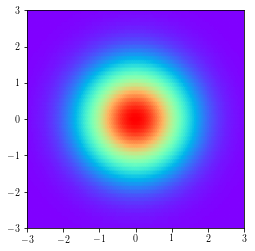
\includegraphics[width=0.24\textwidth]{planar-q0}}
	\subfloat[Planar Flow]{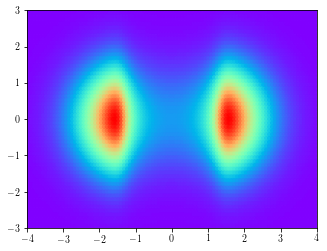
\includegraphics[width=0.31\textwidth]{planar-q1}}
	\subfloat[Radial Flow]{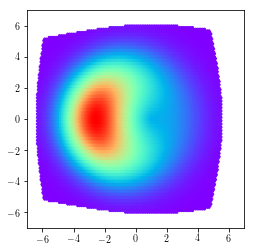
\includegraphics[width=0.24\textwidth]{radial-q1}}
	\caption{Change in standard normal density on application of length 1 planar and radial flows.}
	\label{fig:planarradial}
\end{figure}

\subsubsection{Inverse Autoregressive Flows} Planar and radial flow provide a simple invertible transformation shown to be effective in a low-dimensional latent space (up to hundred dimensions). Equation~\ref{eq:planarfn} of Planar Flow can be seen as Multilayer Perceptron with a single unit bottleneck hidden layer. This means that a long chain of transformations is needed to model a high-dimensional function. 

Autoregressive flows~\cite{germain2015made} is a normalizing flow that scales to high-dimensional latent space by exploiting the ordering f the variables. In autoregressive flow, given a sequence of variable $\mathbf{y} = {y_i}_{i=0}^D$, each variable is only dependent only on variables from the previous index. The distribution is then given by
\begin{align}
p(\mathbf{y}) = \prod_{i=0}^{D} p(x_i | x_0,\dots,x_{i-1})
\end{align} 	 

Kingma et. al.~\cite{kingma2016improved} proposed a Gaussian version of an autoregressive flow on a noise vector $\mathbf{\epsilon} \sim \mathcal{N}(0,\mathbf{I})$ given as follow:
\begin{align}
y_0 &= \mu_0 + \sigma_0 \epsilon_0\\
y_i &= \mu_i(\mathbf{y}_{0:i-1}) + \sigma(\mathbf{y}_{0:i-1}) \epsilon_i\\
\end{align} 

This flow is invertible and the noise $\epsilon$ is given by:
\begin{align}
\epsilon_i &= \frac{y_i - \mu_i(\mathbf{y}_{0:i-1})}{\sigma(\mathbf{y}_{0:i-1})}
\label{eq:iaf}
\end{align} 

Note that, $epsilon$ is independent to each other so the calculation of Equation~\ref{eq:iaf} can be vectorized as follow:
\begin{align}
\bm{\epsilon} &= \frac{\mathbf{y} - \bm{\mu}(\mathbf{y})}{\bm{\sigma}(\mathbf{y})}
\end{align} 
This enables an efficient computation with GPU. 

Due to the autoregressive structure, the transformation has a lower triangular Jacobian where diagonal is $\sigma_i$. For calculation of normalizing flows, we are interested in log-determinant of the Jacobian which is just a product of the diagonal given as:
\begin{align}
\log \det \left| \frac{d\bm{\epsilon}}{d\mathbf{y}} \right| = \sum_{i=0}^{D} - \log \sigma_i(\mathbf{y})
\end{align}

To apply Inverse Autoregressive Flows (IAF) for variational inference in VAE, we add IAF transforms after the latent variables $\mathbf{z}$ and modify the likelihood to account for IAF transforms. Figure~\ref{fig:iaf} shows the process of applying IAF to Variational Autoencoder. 

\begin{figure}[htb]
	\centering
	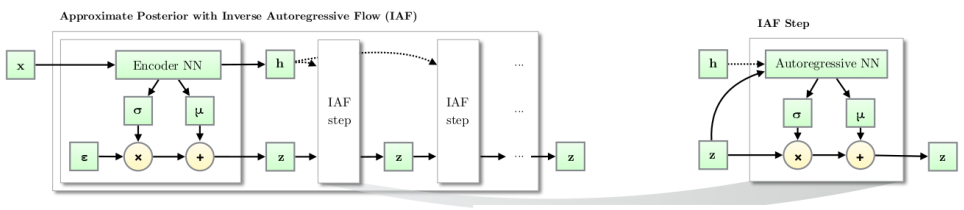
\includegraphics[width=\textwidth]{imgs/iaf}
	\caption{The process of Inverse Autoregressive Flows in Variational Autoencoder~\cite{kingma2016improved}.}
	\label{fig:iaf}
\end{figure}

The flow consists of a chain of $T$ following transformations:
\begin{align}
\mathbf{z}_t = \bm{\mu}_t + \bm{\sigma}_t\mathbf{z}_{t-1}
\end{align}

Kingma et.al.~\cite{kingma2016improved} proposed a more stable update based on LSTM-type update. LSTM is a type of recurrent neural network that applies autoregressive technique to the neural network.  The update is given as follows:
\begin{align}
\mathbf{s}_t &= 1 / \sigma_t\\
\mathbf{m}_t &= -\mu_t / \sigma_t\\
\sigma_t &= sigmoid(\mathbf{s}_t)\\
\mathbf{z}_t &= \sigma_t\mathbf{z}_{t-1} + (1 - \sigma_t)\mathbf{m}_{t} 
\end{align}

where $\bm{\mu}$ and $\bm{\sigma}$ learnt from an Autoregressive neural network given in~\cite{germain2015made} receiving input $\mathbf{z}$ and $\mathbf{h}$ from the VAE. 

\subsection{Density Estimation}
Density Estimation techniques take a different approach from Variational Inference (VI) methods to model the complex data distribution. Unlike VI, these methods aim for exact inference, sampling and log-likelihood evaluation. The primary goal in this regime is to find a bijective function $h=f(x)\;,x \in \mathcal{X}$ to map complex data-distribution $p_X(x)$ to density $p_H(f(x))$. Given that $p_H()$ has a simpler density whose likelihood function is analytically known, the overall log-likelihood of the data can be easily calculated. The complex log-likelihood of the data can now be calculated using the change of variables as follows:
\begin{align}
\log(p_X(x)) = \log(p_H(f(x))) +
\log(\lvert \det(\frac{\partial f(x)}{\partial x}) \rvert) \label{eq:log-likelihood}
\end{align}

\subsubsection{Non-linear Independent Components Estimation} \label{sec:nice}

Non-linear Independent Components Estimation (NICE) \cite{dinh2014nice} is one of the early works adopting normalizing flows in density estimation. This work focuses on transformations $h=f(x)$ that maps the data into a factorized distribution, i.e., the components of $h_d$ are independent. Consequently, the log-likelihood in \cref{eq:log-likelihood} can be written as:
\begin{align}
\log(p_X(x)) = \sum_{d=1}^{D}{\log(p_{H_{d}}(f_{d}(x)))} + \log(\lvert \det(\frac{\partial f(x)}{\partial x}) \rvert)
\end{align}
where $f(x) = (f_{d}(x))_{d \leq D}$.

This work targets invertible functions whose Jacobians have triangular structure so that calculating the determinant is tractable. In particular, it proposes the family of \textit{coupling layers} that we define below.

\paragraph{Coupling layer:} The coupling layer serves a building block of the transformation proposed in this work. The general coupling layer comprises of two partitions $I_{1}, I_{2}$ of the input dimensions  $\left[ 1, D \right]$, such that $d = \lvert I_{1} \rvert$. The transformation is then defined as:

\begin{align}
y_{I_{1}} &= x_{I_{1}} \\
y_{I_{2}} &= g(x_{I_{2}} ; m(x_{I_{1}}))
\end{align}
where
$g: \mathbb{R}^{D-d} \times m(\mathbb{R}^{d}) \rightarrow \mathbb{R}^{D-d}$ is an invertible function. Considering 
$I_{1} = \left[ 1, d \right]$ and $I_{2} = \left[ d, D \right]$,
the Jacobian of this function is:
\begin{align*}
\frac{\partial y}{\partial x} =
\begin{bmatrix}
I_{d} & 0 \\
\frac{\partial y_{I_{2}}}{\partial x_{I_{1}}} & \frac{\partial y_{I_{2}}}{\partial x_{I_{2}}} 
\end{bmatrix}
\end{align*}
Where $I_{d}$ is the identity matrix of size $d$. That means that
$\det \frac{\partial y}{\partial x} = \det \frac{\partial y_{I_{2}}}{\partial x_{I_{2}}}$ which evaluates to $1$. 
The inverse of this transformation can be expressed as:
\begin{align*}
x_{I_{1}} &= y_{I_{1}} \\
x_{I_{2}} &= g^{-1}(y_{I_{2}} ; m(y_{I_{1}}))
\end{align*}
It is important to notice that the inverse of coupling function $m()$ is not required, thus allowing it to be modeled as complex non-linear functions. 
 
\subsubsection{Real-valued Non-Volume Preserving} \label{sec:realnvp}

\section{Normalizing Flows in Probabilistic Programming Languages}
Normalizing flows has been implemented in mainstream probabilistic programming languages that is based on mainstream deep learning framework such as Pyro (based on Pytorch) and Tensorflow Probability (TFP, based on Tensorflow). They provide a construct called the \texttt{Bijector} for the implementation of a function in normalizing flow. We can create our own normalizing function by extending the \texttt{Bijector} construct. TFP also provides a construct called the \texttt{TransformedDistribution} which takes two input a \texttt{Bijector} and the base distribution. \texttt{TransformedDistribution} will run the flow and transform the given base distribution with the given \texttt{Bijector}. There are already numerous function (e.g. Affine, Sigmoid, RealNVP) implemented as a \texttt{Bijector} in TFP. The complete documentation of normalizing flows in TFP is given in this reference~\cite{dillon2017tensorflow}.

To create your own function, you need to extend the \texttt{Bijector} construct and overload these three methods. First, the \texttt{\_forward} function receives samples $x$ from the base distribution as an input and calculate the value of the function $y = f(x)$. Second,  the \texttt{\_inverse} function areceives $y$ from our function as the input nd output $x$ corresponds to the inverse of the function $x = f^{-1}(y)$. Third, the \texttt{\_inverse\_log\_det\_jacobian} function receives $y$ from our function as the input and calculate the inverse log-determinant of the Jacobian $\log \det \left|\frac{\partial f^{-1}}{\partial y}\right|$. After you implement your own function, you can create a list of bijectors corresponds to the flow. TFP provides another bijector called \texttt{Chain} that will chain your list of bijectors into a flow. You can then create an instance of \texttt{TransformedDistribution} with this chain and your base distributor.   

\section{Recent Advances}
In this section, we discuss several recent works that used normalizing flows. We only explain the high-level concept of each work. Interested reader should refer to the original paper given in the reference.
\subsection{Pixel Recurrent Neural Network}
Pixel Recurrent Neural Network (PixelRNN)~\cite{oord2016pixel} is an auto-regressive image generative model where the joint distribution over the image pixel is factorized into a product of conditional distribution. This means that the probability of pixel at position $i$ is given as: $p(x_i | x_1, \dots, x_{i-1})$ where $x_1, \dots, x_{i-1}$ is the previously generated pixels. This is a strong and counter-intuitive assumption for an image generation where pixel mostly conditioned on their neighbors. However, PixelRNN is proven to  work well for image completion and generation task. In image completion, the occluded pixel is generated by conditioned upon the non-occluded pixels.

Oord et. al.~\cite{oord2016pixel} proposed three methods model an auto-regressive image generation.  First, Row LSTM 1D convolution is used to generate image row by row from top to bottom. However, Row LSTM cannot capture the whole previously generated pixels since there is a coarse-graining in the convolution method. Second, Bidirectional LSTM is used to capture all the generated pixels as the context. Every pixel is conditioned upon their neighboring pixels except the one that has not been generated. However, LSTM training is known to be expensive so the authors proposed another model based on CNN. Third, Pixel CNN used a masked convolution by setting the filter of the pixels that has not been generated as zero.

% Each method is visualize in Figure~\ref{fig:pixelrnn}. 
%\begin{figure}[htb]
%	\centering
%	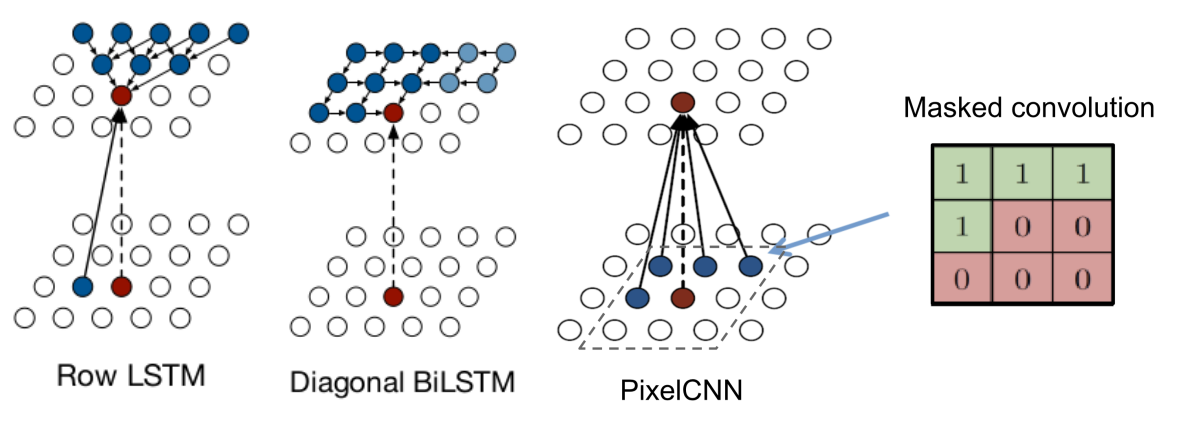
\includegraphics[width=\textwidth]{imgs/pixelrnn}
%	\caption{The process of Inverse Autoregressive Flows in Variational Autoencoder~\cite{kingma2016improved}.}
%	\label{fig:pixelrnn}
%\end{figure}

\subsection{Wavenet}
Wavenet~\cite{van2016wavenet} used the idea of Pixel CNN from~\cite{oord2016pixel} for raw audio generation. It used one-dimensional convolution Pixel CNN to generate raw audio. Wavenet has been proven to be the state-of-the-art model for text-to-speech model. Google Assistant in Android use wavenet to generate the audio of the assistant. 

Similar to Pixel CNN, the joint probability of an input audio is modelled by a stack of causal convolutional layers. Causal convolution has similar idea to masked convolution by shifting the output of a normal convolution by a few timesteps so it does not violate the autoregressive requirement. One of the problems with causal convolution is that it requires deep layers to capture long range dependency. The authors proposed to use dilated convolution where the convolution filter is applied over an area larger than its length. This is done by skipping input values with a certain step. 

\subsection{Glow}
Glow~\cite{kingma2018glow} extended and simplified the NICE and RealNVP model explained in Section~\ref{sec:realnvp} with three main extensions. First, the authors used activation normalization (act-norm) instead of batch normalization in RealNVP.  Act-norm performs a channel-wise normalization and is faster than batch normalization. Second, the authors used $1\times1$ convolution for the channel-wise permutation. NICE and RealNVP proposed a flow containing the equivalent of a permutation that reverses the ordering of the channels. This is changed with a $1\times1$ convolution so that the permutation can be learned.  Third, they extend RealNVP so that it can work faster by changing it into a multi-scale architecture. The authors splitted each step of the flow so it can be parallelized.

All of the additions mentioned before can be inverted and log-determinant of the Jacobian can be computed easily. Please refer to the paper for the details of the inversion and calculation of the Jacobian matrix. Glow has similar advantage as RealNVP that it can generate a high quality images. Moreover, the latent space learned by Glow is meaningful. This means that we can control the output of the generated image by tuning the latent space.


\section{Conclusion}
%
% ---- Bibliography ----
%
% BibTeX users should specify bibliography style 'splncs04'.
% References will then be sorted and formatted in the correct style.
%
% \bibliographystyle{splncs04}
% \bibliography{mybibliography}
%
\bibliographystyle{splncs04}
\bibliography{ref} 




\appendix


\section{Appendix (Contribution)}
\textbf{Abdul Fatir Ansari}
\begin{enumerate}
	\item 
\end{enumerate}

\textbf{Devamanyu Hazarika}
\begin{enumerate}
	\item 
\end{enumerate}


\textbf{Remmy A. M. Zen}
\begin{enumerate}
	\item Inverse autoregressive flows subsection.
	\item Recent advances section.
	\item Normalizing flows in PPL.
\end{enumerate}

\section{Appendix (Abdul Fatir Ansari)}


The Jacobian is then given by

\begin{align*}
\frac{\partial f(\mathbf{z})}{\partial \mathbf{z}} = \mathbf{I} + \mathbf{u}h'(\mathbf{w}^\top\mathbf{z} + b)\mathbf{w}^\top
\end{align*}

Now, using the matrix determinant lemma

\begin{align}
\det\frac{\partial f(\mathbf{z})}{\partial \mathbf{z}} &= (1 + h'(\mathbf{w}^\top\mathbf{z} + b)\mathbf{w}^\top\mathbf{I}^{-1}\mathbf{u})\det(\mathbf{I})\\
&=(1 + h'(\mathbf{w}^\top\mathbf{z} + b)\mathbf{w}^\top\mathbf{u})\label{eq:planar-det}
\end{align}

\section{Appendix (Devamanyu Hazarika)}
\section{Appendix (Remmy Zen)}

\end{document}
